\chapter{Bezprzewodowe sieci czujnikowe}
Bezprzewodowe sieci czujnikowe są systemami składającymi się dużej liczby węzłów, z których każdy wyposażony w moduły umożliwiające gromadzenie, przetwarzanie oraz przesyłanie informacji \cite{Ilyas2004}, dzięki czemu możliwe staje się obserwowanie oraz reagowanie na zdarzenia występujące w objętym jej zasięgiem środowisku. Środowiskiem tym może mieć charakter zarówno fizyczny, jak też i biologiczny czy stanowić fragment systemu informatycznego. 
\cite{Sohraby2006}
Bezprzewodowa sieć czujnikowa składa się z czterech podstawowych elementów\cite{}:
\begin{enumerate}
	\item Zestawu czujników rozmieszczonych na określonym obszarze
	\item Sieci łączącej te czujniki
	\item Co najmniej jednego węzła gromadzącego dane z pozostałych
	\item Węzłów lub zewnętrznej do sieci jednostki, której zadaniem jest przetworzenie zebranych danych
\end{enumerate}
Wartym odnotowania jest fakt, że przetwarzanie danych może się odbywać w samej sieci czujników, bez konieczności udziału zewnętrznych jednostek.

Sieci czujnikowe są najczęściej same organizują swoją strukturę. Oznacza to, że hierarchia (lub jej brak) sieci oraz trasy pakietów są dynamicznie wypracowywane przez węzły sieci zgodnie z zaimplementowanymi protokołami.
Do innych wyróżniających te sieci charakterystyk należą ograniczenia związane z dostępem do energii elektrycznej, czasem życia baterii, redundancja danych krążących w sieci oraz kolizje pakietów.

Przykładami zastosowań są gromadzenie danych, monitoring, telemetria medyczna \cite{Biradar2009}.

Czujnik z technicznego punktu widzenia jest urządzeniem, którego zadaniem jest zbieranie informacji o obiektach i procesach fizycznych wraz ze zmianami ich stanu.\cite{Dargie2010}

W celu stworzenia sieci czujników konieczne jest wcześniejsze zaprojektowanie i stworzenie pojedynczego węzła. Bardzo często narzucone są na nie dodatkowe ograniczenia: wielkość, pobór energii, koszt wytworzenia. Dodatkowo muszą posiadać odpowiednie czujniki, moduły komunikacyjne oraz moc obliczeniową odpowiednią do ich obsłużenia. W książce \cite{Karl2006} architekturę sprzętową pojedynczego węzła rozbito na pięć komponentów:
\begin{enumerate}
	\item Sterownik - komponent odpowiedzialny za zbieranie danych z czujników oraz ich przetwarzanie. Ponadto decyduje on kiedy oraz gdzie wysłać te dane oraz steruje zachowaniem aktuatorów. Funkcje te realizuje dzięki wykonywaniu instrukcji zawartych w kodzie uprzednio napisanych programów. Sterownik można zrealizować wykorzystując różne architektury układów scalonych. Najczęściej używane są mikrokontrolery. Głównymi ich zaletami są łatwość w komunikacji z urządzeniami zewnętrznymi takimi jak np. czujniki, niski pobór energii (mogą zostać również przełączone w tryb uśpienia) oraz łatwa programowalność.
	\item Pamięć - komponent przechowujący programy oraz dane. Do przechowywania odczytów z czujników przed wysyłką lub przetworzniem oraz odebranych pakietów wykorzystuje się pamięć RAM. Programy zapisywane są w pamięci ROM, EEPROM lub Flash. Pamięć Flash bywa również używana do przechowywania pomiarów w sytuacjach, gdy pamięć RAM okazuje się niewystarczająca lub w celu zapisu danych z pamięci RAM przed wyłączeniem czujnika.   
	\item Czujniki i aktuatory - urządzenia zbierające informacje o środowisku zewnętrznym oraz urządzenia wpływające na jego stan. Mogą to być między innymi czujniki wielkości elektrycznych, pola magnetycznego, wykrywacze fal radiowych, czujniki optyczne, elektrooptyczne, podczerwieni, lasery, radary, lokalizacyjne, fal sejsmicznych, badające parametry środowiskowe (pęd wiatru, temperaturę, wilgotność, ciśnienie), biochemiczne \cite{Sohraby2006}.
	\item Komunikacja - komponent odpowiedzialny za wysyłanie oraz odbieranie danych za pośrednictwem bezprzewodowego kanału komunikacyjnego. Najczęściej wykorzystywanym medium są fale radiowe - umożliwiają one wysyłanie danych na relatywnie długie dystanse przy małym zużyciu energii. 
	\item Zasilanie - najczęściej są to baterie lub ogniwa słoneczne
\end{enumerate}

\begin{figure}[H]
	\begin{center}
		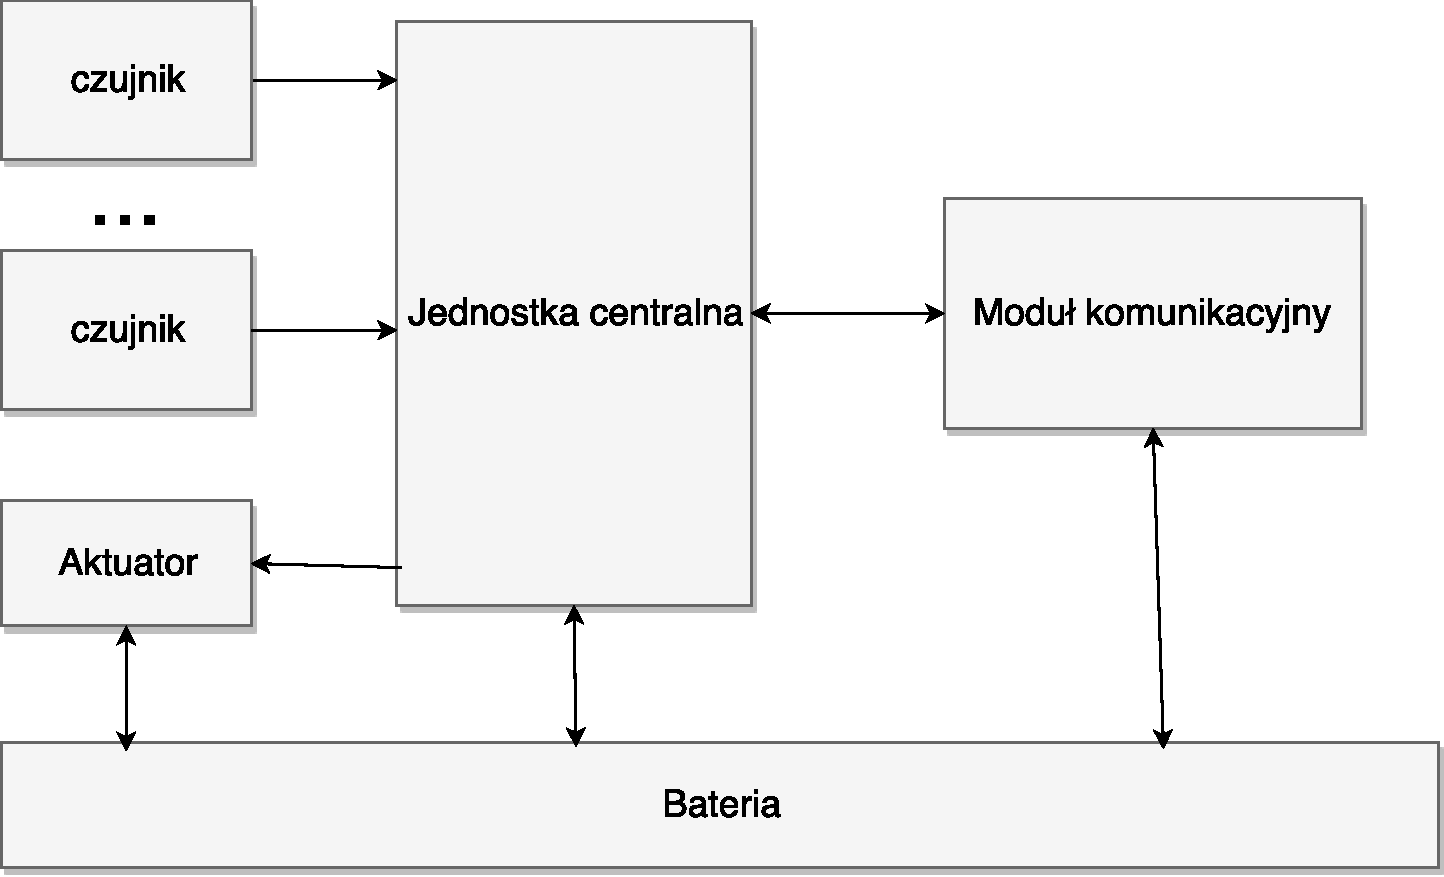
\includegraphics[scale=0.5]{\ImgPath/sensor_node.pdf}
	\end{center}
	\caption{Architektura węzła sieci czujnikowej}
\end{figure}

\section{Trasowanie w WSN}
Bezprzewodowe sieci czujnikowe mają wiele wspólnego z sieciami przewodowymi i ad-hoc, jednakże wykazują również swoje własne, unikatowe cechy oraz związane z nimi wyzwania.
Jedną z takich cech jest różnorodna gęstość sieci oraz liczba węzłów. Sieci czujnikowe mogą składać się z od kilkuset do kilku tysięcy węzłów rozmieszczonych w sposób losowy o różnorodnym zagęszczeniu. Zachowanie tych węzłów jest dynamiczne, jako że do ich zadań oprócz zbierania danych oraz przesyłania pakietów należy również oszczędzanie własnej energii. Dodatkowo duży wpływ na jakość połączenia mają wysokie poziomy szumu oraz interferencja.
Istotnym wyzwaniem związanym z sieciami czujników jest również model danych oraz ich przepływu, który różni się w zależności od konkretnego rozwiązania, w którym sieć jest wykorzystywana. Węzły sieci mogą cyklicznie wysyłać do stacji bazowej próbkę danych. W modelu zdarzeniowym węzeł sieci wysyła pakiet po wystąpieniu określonego zjawiska. Istnieją również implementacje wymagające od węzłów sieci przetwarzania oraz agregacji danych przez węzeł przed ich wysyłką, czy takie, które wymagają komunikacji dwukierunkowej pomiędzy węzłami a stacją bazową.

%Więcej wyzwań z Routing Protocols in Wireless Sensor Networks –
%A Survey

Taka różnorodność modeli przepływu danych oraz innych wyzwań wymagają zastosowania odpowiednio zoptymalizowanych algorytmów trasowania \cite{Abdullah2014, Sohraby2006}.

Z powodu różnych potrzeb odnośnie trasowania pakietów zaproponowany został szereg metryk dotyczących zasobów sieci. Celem protokołów trasowania jest optymalizacja ich wykorzystania \cite{Dargie2010, Biradar2009}.

Minimalizacja ścieżki pakietu do węzła bazowego

Minimalizacja energii zużytej na wysłanie pakietu

Maksymalizacja czasu, po którym następuje podział sieci

Minimalizacja wariancji poziomów energii węzłów


\subsection{Flood}
Węzeł wysyłający pakiet rozgłasza go do najbliższych sąsiadów, którzy z kolei powtarzają ten krok, aż pakiet nie dotrze do wszystkich węzłów sieci lub nie osiągnie maksymalnej liczby skoków.
W przypadku tego algorytmu, jeżeli istnieje droga łącząca źródło pakietu z celem, to cel z pewnością go otrzyma.
Zaletą tego algorytmu jest jego prostota. Do wad natomiast zalicza się duży ruch pakietów w sieci. W celu jego ograniczenia oraz zapewnienia aby pakiet nie był wysyłany w nieskończoność stosowane są dwa mechanizmy \cite{Dargie2010}:
\begin{itemize}
	\item maksymalna liczba przeskoków pakietu
	\item numery sekwencji pakietów - pakiety otrzymują kolejne numery, które wraz z adresem węzła wysyłającego umożliwiają jego identyfikację. Dzięki temu węzły mogą przechowywać historię otrzymanych (oraz rozgłoszonych dalej pakietów) i w momencie w którym taki pakiet ponownie otrzymają - go odrzucić.
\end{itemize}

Mechanizmy te jednakże nie rozwiązują następujących problemów występujących w protokole Flood \cite{Dargie2010}:
\begin{itemize}
	\item Implozja - węzeł, który otrzymał pakiet rozgłasza go do swoich sąsiednich węzłów niezależnie od tego, czy otrzymały one już ten pakiet od innego węzła. Prowadzi to do niepotrzebnego zużycia zasobów. %Dorzucić obrazek
	\item Redundancję geograficzną - pakiety wysyłane przez węzły monitorujące pokrywające się obszary są traktowane jako kompletnie od siebie różne (brak fuzji danych), co prowadzi do marnowania zasobów (ta sama informacji wysyłana jest wielokrotnie). %Dorzucić obrazek
	\item Nieuwzględnianie zasobów węzła - ze względu na swoją prostotę algorytm nie bierze pod uwagę aktualnych zasobów węzła sieci.
\end{itemize}
\subsection{SPIN}
Protokół SPIN (Sensor Protocols for Information via Negotiation) jest rodziną protokołów trasowania typu płaskiego. Do rozsyłania informacji po sieci wykorzystują negocjację. Do ich przeprowadzenia wykorzystują pakiety zawierające metadane opisujące przesyłane wiadomości. Dzięki temu możliwe jest wyeliminowanie redundancji transmisji występujące w protokołach typu Flood \cite{Chaudhary2015}.

Projekt protokołów SPIN wyrósł z protokołów Flood. Twórcy zauważyli trzy podstawowe problemy w tego typu podejściu:
\begin{itemize}
	\item Implozję
	\item Redundancję geograficzną
	\item Nieuwzględnianie zasobów
\end{itemize}

Innowacjami w stosunku do protokołu Flood są negocjacja oraz adaptacja w zależności od zasobów.

\paragraph{Negocjacja} W celu rozwiązania problemów związanych z implozją oraz przenikaniem się monitorowanych obszarów, przed wysłaniem pakietu węzły negocjują między sobą. Do negocjacji wykorzystywane są dodatkowe informacje o pakietach - meta-dane. 
Meta-dane wykorzystywane są do precyzyjnego opisu danych zbieranych przez czujniki. Rozmiar w bajtach meta-danych musi być mniejszy od rozmiaru samego pakietu z danymi, aby rozwiązanie miało sens.
Sam protokół nie narzuca tego co meta-dane powinny zawierać. Jest to zależne od konkretnego rozwiązania oraz implementacji. Może to być np. identyfikator węzła, współrzędne geograficzne, itd. Specyfikacja, przechowywanie oraz przetwarzanie meta-danych wykracza poza algorytm SPIN.
W protokole SPIN węzły komunikują się za pomocą trzech rodzajów pakietów:
\begin{itemize}
	\item ADV - ogłoszenie nowych danych. Jest to pakiet zawierający meta-dane. Ogłasza on węzłom pojawienie się nowych danych
	\item REQ - zgłoszenie zamówienia na dany pakiet z danymi. Węzeł, który chce otrzymać konkretny pakiet wysyła wiadomość z jego meta-danymi (tymi, które otrzymał w ADV)
	\item DATA - pakiet zawierający właściwe dane z czujnika wraz z meta-danymi
\end{itemize}
Przebieg negocjacji ilustruje poniższy schemat:
\begin{figure}[H]
	\begin{center}
		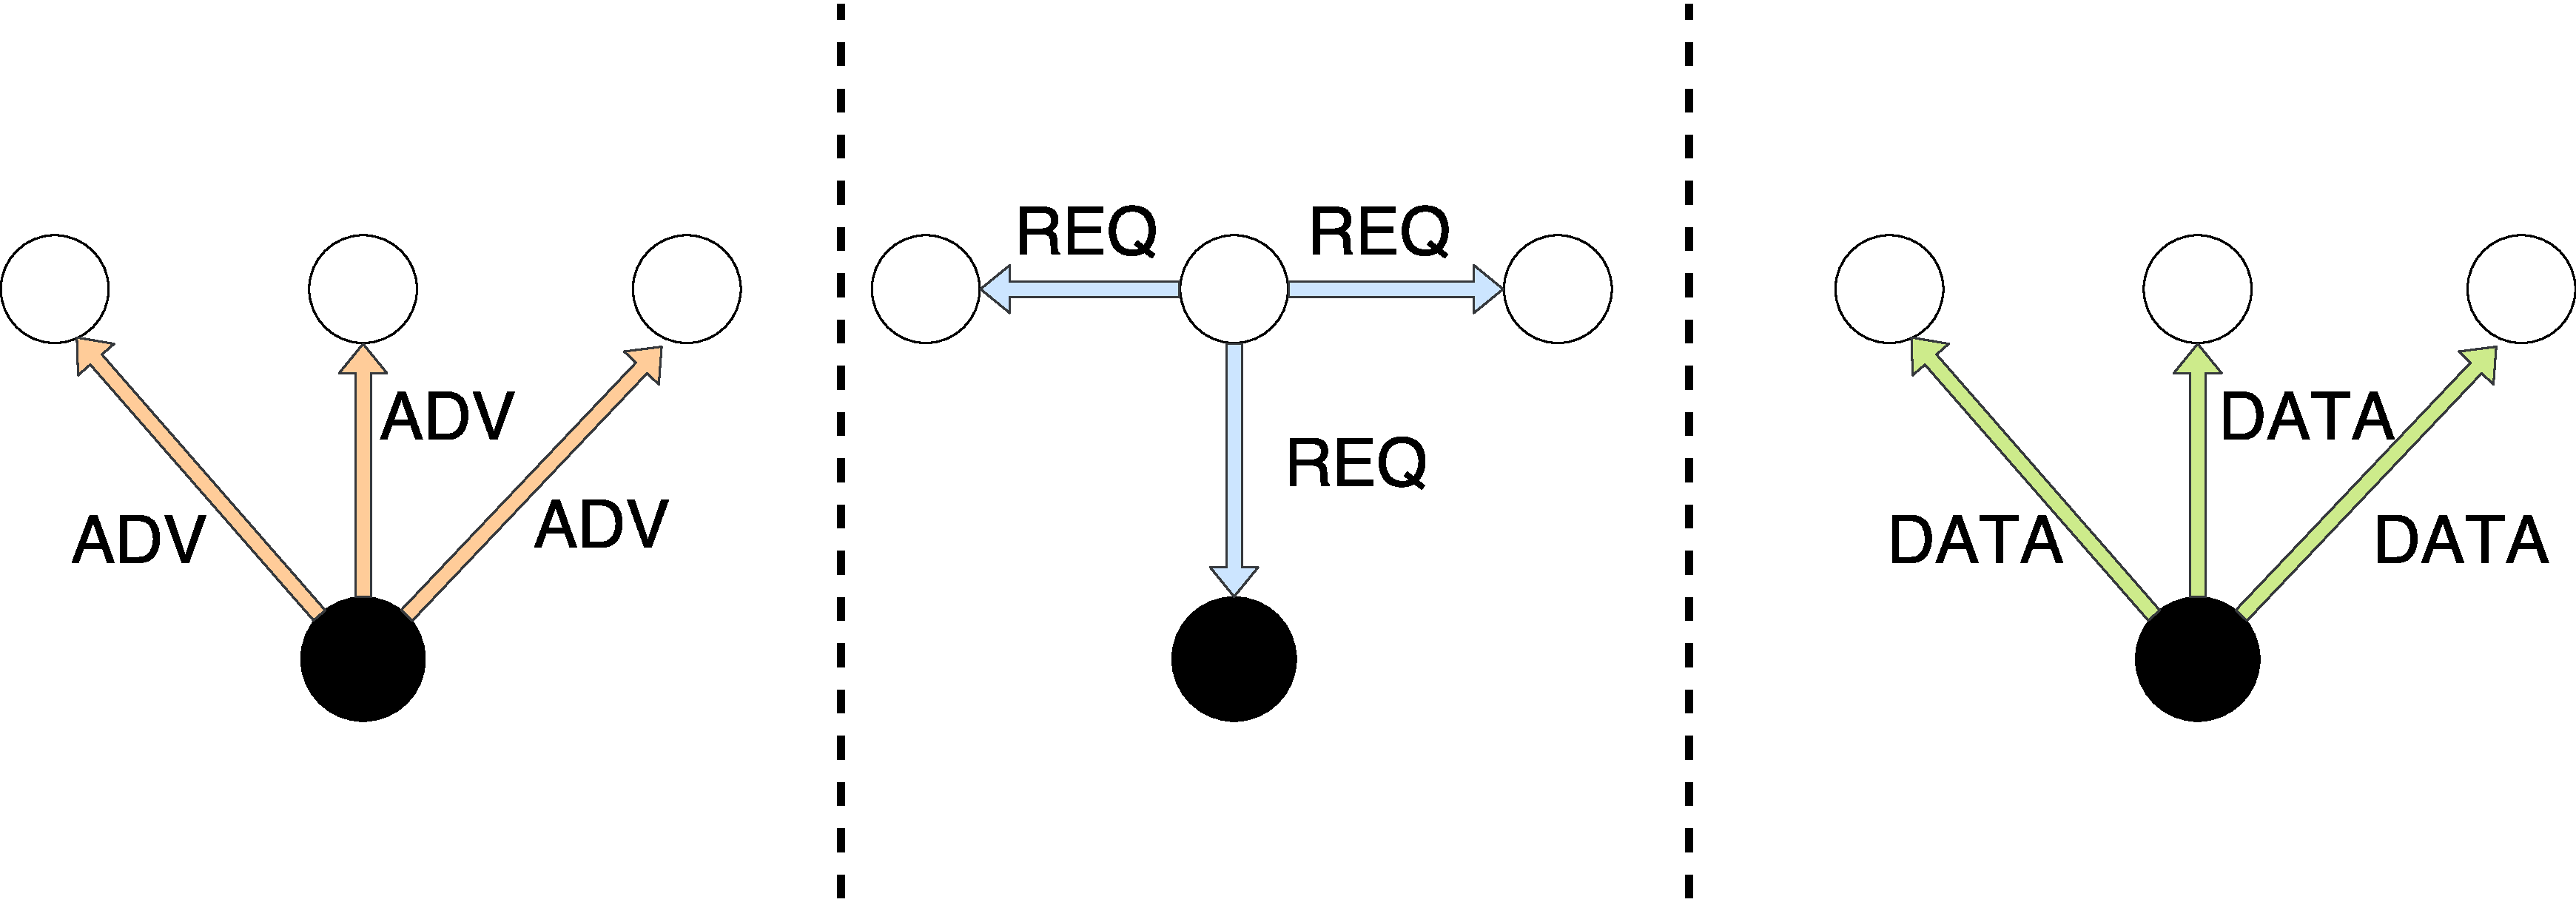
\includegraphics[scale=0.25]{\ImgPath/protocols/spin.pdf}
	\end{center}
	\caption{Przebieg negocjacji w protokole SPIN}
\end{figure}

Jako, że pakiety ADV i REQ zawierają tylko meta-dane, są one tańsze do wysłania niż DATA.

W skład rodziny algorytmów SPIN wchodzą cztery protokoły: SPIN-PP, SPIN-EC, SPIN-BC, SPIN-RL. Jako, że protokoły SPIN-PP oraz SPIN-EC nie przeznaczone są dla sieci point-to-point, opisane zostaną dwa pozostałe protokoły \cite{Dargie2010, Kulik2002}.

Protokół zaczyna się od wysłania pakietu ADV przez węzeł, który posiada nowe dane, które chce rozpropagować w sieci. Węzły sąsiednie, które otrzymały wiadomość ADV, sprawdzają czy otrzymały już takie dane. Jeśli reklamowane dane są dla nich nowe, wysyłają one wiadomość REQ z powrotem do nadawcy. Węzeł inicjujący negocjację po otrzymaniu wiadomości REQ wysyła dane w pakiecie DATA

\subparagraph{SPIN-BC}
W tym wariancie wykorzystany jest fakt, że węzły współdzielą medium komunikacyjne. Komunikacja pomiędzy dwoma węzłami może zostać ''podsłuchana'' przez węzły znajdujące się w zasięgu. Wszystkie pakiety wysyłane są w trybie rozgłoszeniowym, jako że dla sieci bezprzewodowej nie wiąże się to z dodatkowym kosztem.

Wiadomość ADV jest rozgłaszana do wszystkich sąsiednich węzłów. Jednakże przed wysłaniem wiadomości REQ węzły czekają przez losowy okres. Jeżeli węzeł przechwycił wiadmość REQ dotyczącą tych samych danych, których i on potrzebuje, anuluje on wysyłkę swojej wiadomości REQ (nie jest potrzebna, redukuje to koszty). Pozwala to również na uniknięcie kolizji. Po otrzymaniu REQ węzeł wysyła pakiet DATA do kanału rozgłoszeniowego. Pakiet DATA jet wysyłany tylko raz, następujące po nim wiadomości REQ dotyczące tych samych danych są ignorowane.
\subparagraph{SPIN-RL}
SPIN-RL jest przystosowaniem SPIN-BC do warunków komunikacji stratnej. Każdy węzeł przechowuje listę wiadomości ADV i jeśli nie otrzyma on danych w odpowiednim czasie, to ponawia on wysyłkę zapytania o dane (REQ). Odbiorca jest losowany z listy węzłów które wysłały ogłoszenie o tych samych danych.
Po wysyłce pakietu DATA musi upłynąć pewien odstęp czasowy przed ponowną wysyłką.

%Zakończenie
Zgodnie z badaniami opisanymi w artykule \cite{Kulik2002} protokoły SPIN są w stanie dostarczyć 60\% więcej danych w sieciach point-to-point i 80\% więcej danych w sieciach rozgłoszeniowych niż tradycyjne rozwiązania.  
\subsection{LEACH} \label{subsec:leach}
LEACH jest protokołem typu hierarchicznego, który wykorzystuje dwa poziomy grupowania węzłów. Pakiety trasowane są od czujników do Cluster Headów i od Cluster Headów do stacji bazowej \cite{Yu2006}.
Węzły same organizują się w klastry, w których jeden węzeł pełni funkcję lokalnego węzła bazowego - nazywany jest on również Cluster Head. W przeciwieństwie do konwencjonalnych algorytmów lokalne węzły bazowe nie są wybierane a priori. Wybierane są rotacyjnie w sposób losowy, tak aby równomiernie rozłożyć zużycie energii oraz wybierać węzły z możliwie jak największą energią. Dodatkowo LEACH wykorzystuje fuzję danych w celu skompresowania ich ilości przesyłanych z klastra do stacji bazowej \cite{Akkaya2005}%\cite{Heinzelman00}.

Działanie algorytmu podzielone jest na rundy. Każda runda składa się z fazy konfiguracyjnej, po której następuje faza stabilnego działania sieci. W fazie początkowej każdy węzeł decyduje o tym czy ma zostać lokalnym węzłem bazowym w aktualnej rundzie. Decyzja ta opiera się na zadanej przez użytkownika liczbie lokalnych węzłów bazowych w sieci (wyrażonej jako procent od liczby wszystkich węzłów sieci) oraz na fakcie uprzedniego bycia lokalnym węzłem bazowym.
Algorytm ten przebiega w sposób następujący:
\begin{enumerate}
	\item Węzeł n losuje liczbę z zakresu od 0 do 1
	\item Obliczany jest próg wyrażony poniższym wzorem
	\[T(n) = \begin{dcases} 
      \frac{P}{1-P*(r\:mod\frac{1}{P})} & n \in G \\
      0 & n \not\in G \\
   \end{dcases}
	\]
	, gdzie P - procent sieci, którą powinny stanowić lokalne węzły bazowe,
	r - numer aktualnej rundy
	G - zbiór węzłów, które nie były lokalnymi węzłami bazowymi przez ostatnie $\frac{1}{P}$ rund.
	\item Jeżeli wylosowana liczba jest mniejsza od progu $T(n)$, to węzeł zostaje lokalnym węzłem bazowym.
\end{enumerate}
Taki wybór lokalnych węzłów bazowych gwarantuje, że każdy węzeł sieci zostanie nim w ciągu $\frac{1}{P}$ rund. Wszystkie węzły, które zostały wybrane jako lokalne węzły bazowe w pierwszej rundzie (o numerze 0) nie zostaną nimi przez kolejnych $\frac{1}{P}$ rund. Przez kolejne rundy wartość progu $T(n)$ rośnie. Funkcja została zaprojektowana w ten sposób, aby wraz ze zmniejszaniem się liczby węzłów, które mogą zostać potencjalnie wybrane na lokalne węzły bazowe prawdopodobieństwo ich wyboru rosło. Po $\frac{1}{P}$ rundach próg $T(n)$ wraca do stanu początkowego, tym samym rozpoczynając ponownie opisany cykl.
Powyższy algorytm zakłada, że wszystkie węzły są homogeniczne pod względem początkowej ilości energii oraz jej zużycia.

Węzeł, który został wybrany na lokalny węzeł bazowy ogłasza ten fakt  pozostałym węzłom. Wykorzystywany jest przy tym protokół MAC CSMA. W tym czasie pozostałe węzły sieci muszą mieć włączone odbiorniki radiowe. Po zakończeniu tej fazy każdy z węzłów sieci nie będący lokalnym węzłem bazowym dokonuje decyzji, do którego klastra będzie należeć. Wybrany zostaje ten klaster, od którego zostało otrzymane ogłoszenie o największym wskaźniku mocy odebranego sygnału (z ang. RSSI - Received Signal Strength Indication). Dzięki tymi wybrany zostaje lokalny węzeł bazowy, z którym komunikacja jest najmniej kosztowna energetycznie.

Po dokonaniu wyborów klastrów przez węzły muszą one ów wybór zakomunikować lokalnym węzłom bazowym. Wysyłają więc one pakiet informujący o dołączeniu do klastra lokalnym węzłom bazowym (również z wykorzystaniem protokoły MAC CSMA).

Po otrzymaniu informacji zwrotnej od węzłów, lokalne węzły bazowe tworzą harmonogramy TDMA na podstawie liczby węzłów w klastrze. Z pozostałego czasu rundy przeznaczonego na fazę stabilną wydzielane są dla każdego węzła przedziały czasowe, podczas których mogą one wysłać swoje pakiety z danymi do lokalnego węzła bazowego. Harmonogram zostaje rozgłoszony do wszystkich węzłów w klastrze.

Po utworzeniu klastrów oraz harmonogramów TDMA, następuje faza stabilnego działania sieci, podczas której węzły przesyłają zebrane dane do lokalnych węzłów bazowych. Każdy węzeł transmituje pakiety w wyznaczonym dla niego przedziale czasowym. Transmisja odbywa się przy użyciu minimalnej energii, tak aby pakiet mógł dotrzeć do lokalnego węzła bazowego. Pozostałe węzły w klastrze (nie biorące udziału w transmisji) mogą w tym czasie wyłączyć odbiorniki radiowe w celu konserwacji energii. Po otrzymaniu pakietu z danymi, lokalny węzeł bazowy przetwarza go oraz agreguje zgodnie z zaimplementowanymi regułami. Sposób kompresji oraz agregacji sygnałów jest dostosowywany do specyfiki danych zbieranych przez sieć (np. dane o temperaturze mogą zostać uśrednione). Po zebraniu danych lokalny węzeł bazowy przesyła je w pakiecie do stacji bazowej, po czym następuje nowa runda.
\begin{figure}[H]
	\begin{center}
		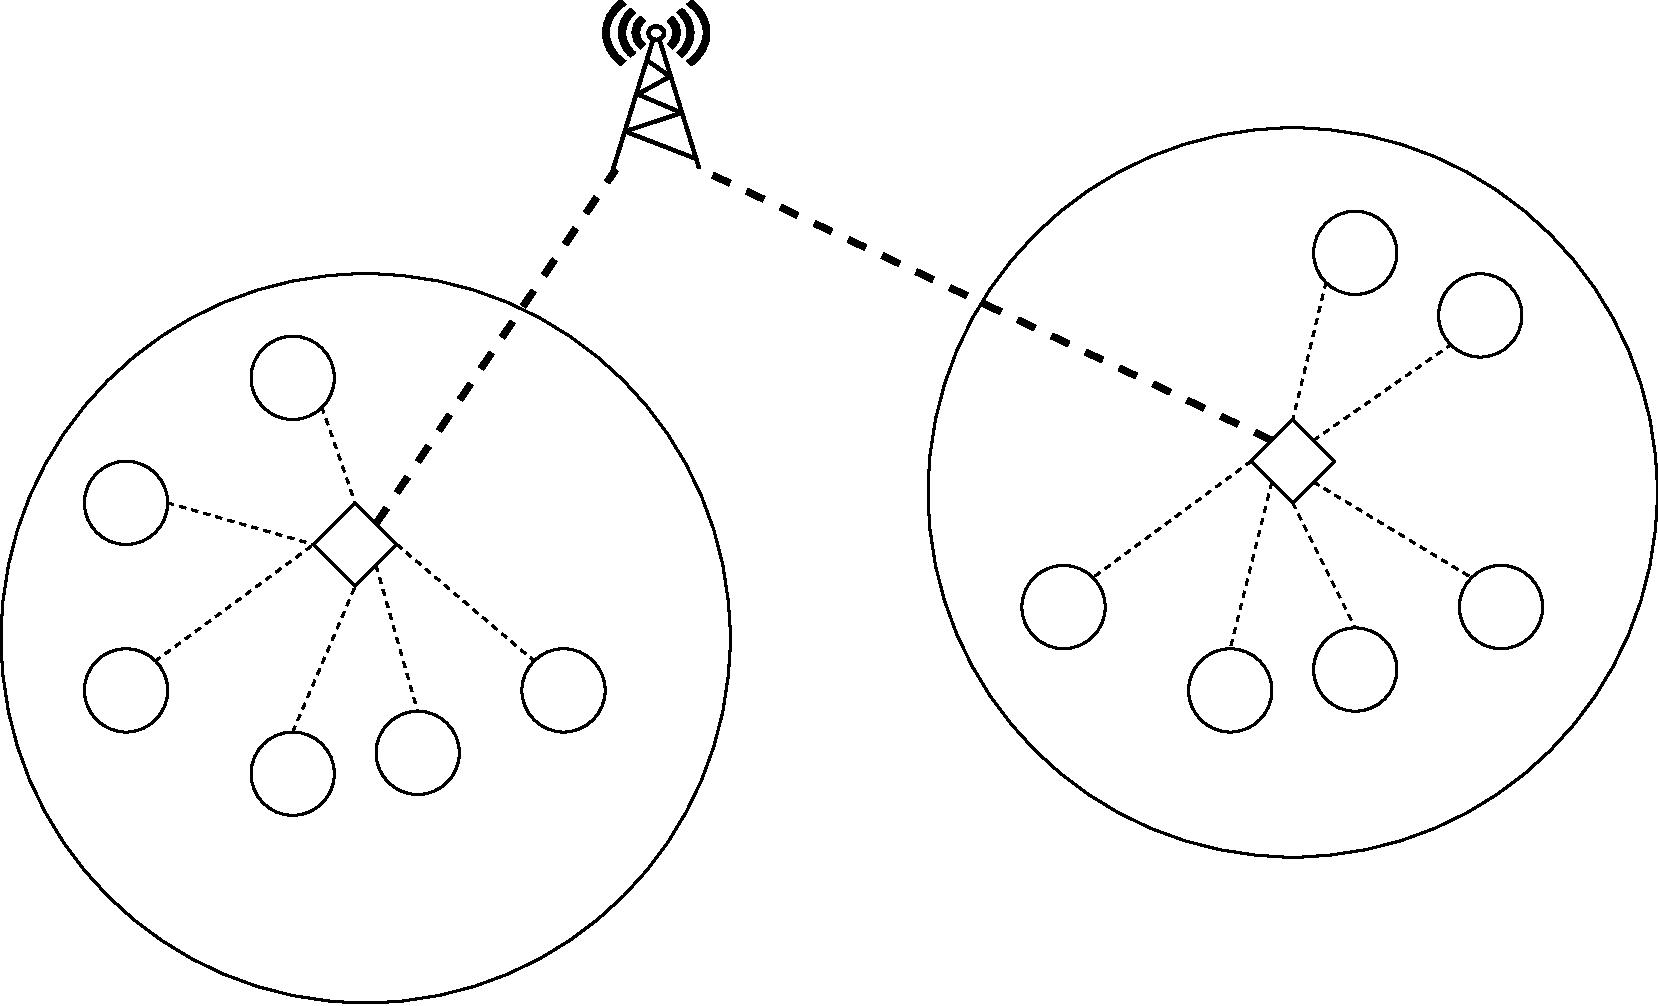
\includegraphics[scale=0.3]{\ImgPath/protocols/leach.pdf}
	\end{center}
	\caption{LEACH}
\end{figure}
\paragraph{ALEACH (Advanced LEACH)} \label{para:aleach}
ALEACH zmienia sposób wyboru lokalnego węzła bazowego. Nowy sposób obliczania progu $T(n)$ opiera się na nowych parametrach nazwanych prawdopodobieństwem aktualnego stanu oraz globalnym prawdopodobieństwie \cite{Ali2008}.

\[
	T(n) = G_{p} + CS_{p}
\]

Prawdopodobieństwo aktualnego stanu ($CS_{p}$) wyrażone jest poniższym wzorem \cite{Ali2008}.
\[
	CS_{p} = \frac{E_{aktualne}}{E_{n-max}}*\frac{K}{N}
\]
Gdzie $E_{aktualne}$ oznacza aktualną energię węzła, $E_{n-max}$ stanowi początkową energię sieci, $K$ spodziewaną liczbę lokalnych węzłów bazowych w rundzie, a $N$ liczbę wszystkich węzłów sieci. Im większa energia rezydualna w danym węźle, tym większe jest prawdopodobieństwo, że zostanie on lokalnym węzłem bazowym.

Prawdopodobieństwo globalne natomiast liczone jest zgodnie ze wzorem \cite{Ali2008}:
\[
	G_{p} = \frac{K}{N - K * (r \:mod \frac{N}{K})}
\]

Pozostała część algorytmu jest taka sama jak w LEACH. Dzięki uwzględnieniu podczas wyboru lokalnego węzła bazowego jego aktualnej energii algorytm ten pozwala na wydłużenie życia sieci w stosunku do LEACH \cite{Singh2017}.
\paragraph{LEACH DCHS (LEACH-Deterministic Cluster Head Selection)}
Celem tego wariantu protokołu LEACH, tak samo jak w przypadku ALEACH, jest wydłużenie działania sieci czujników. Efekt ten został uzyskany dzięki modyfikacji progu $T(n)$ \cite{Handy2002, Singh2017}.
 \[
	T(n) =  \frac{P}{1 - P * (r \:mod \frac{1}{P})} * \left[\frac{E_{n_{aktualne}}}{E_{max}} + \left(r_{s} \backslash \frac{1}{p}\right)\left(1 - \frac{E_{n_{aktualne}}}{E_{max}}\right)\right]
\]